%%=============================================================================
%% Selectie
%%=============================================================================
\chapter{\IfLanguageName{dutch}{Proof-of-concept}{Proof-of-concept}}%
\label{ch:proof-of-concept}

In dit hoofdstuk wordt de proof-of-concept besproken 
waarbij een beoordeling wordt gevormd van de omgevingen op basis van de performantie metingen.
Allereerst wordt de opzet van de proof-of-concepts voor beide omgevingen besproken.
Hierna worden de performantie metingen uitgevoerd voor beide omgevingen waarna de resultaten worden besproken.
Als laatste worden alle resultaten samengevat in de discussie sectie om zo te bekijken of Bun een geschikte plaatsvervanger
van Node.js kan zijn.

\subsection{Opzet proof-of-concept}
Voor de performantie te meten worden er per omgeving 2 proof-of-concepts gemaakt. 
Deze metingen zullen worden uitgevoerd op een Mac mini met volgende specificaties:
\begin{itemize}
  \item De Apple M2 chip.
  \item 8GB aan unified memory.
  \item Het macOS Sonoma besturingssysteem
  \item 256GB aan SSD opslag.
  \item Versie 21 van Node.js.
  \item Versie 1.1.3 van Bun.
\end{itemize}
De eerste proof-of-concept zal bestaan uit een script dat het QuickSort algoritme bevat. 
Deze zal dienen om de computationele verwerking van elke omgeving te beoordelen. 
Hierbij wordt rekening gehouden met de gemiddelde uitvoeringstijd en het maximale geheugengebruik.
Het QuickSort algoritme zal een meegegeven array sorteren door een spil element te kiezen binnen de array
waarna de array in twee wordt opgesplitst. De eerste array zal elementen bevatten die kleiner zijn dan het spil element 
en de andere array zal elementen bevatten die groter zijn. 
De 2 arrays worden vervolgens telkens recursief gesorteerd met dezelfde methode om zo een gesorteerde array te bekomen.
In het codevoorbeeld ~\ref{code:quicksort} kan de code voor het QuickSort algoritme gevonden worden.
Hierbij is er de mogelijkheid de grootte van de te sorteren array mee te geven via de command-line.

\begin{listing}[H]
    \centering
    \begin{minted}[bgcolor=bg,
        fontfamily=tt,
        linenos=true,
        numberblanklines=true,
        numbersep=5pt,
        gobble=0,
        framesep=2mm,
        tabsize=4,
        obeytabs=false,
        breaklines=true,
        mathescape=false
        samepage=false,
        showspaces=false,
        showtabs =false,
        texcl=false]{js}
const quickSort = (array) => {
  if (array.length <= 1) {
    return array;
  }

  let pivot = array[0];
  let smallArray = [];
  let bigArray = [];

  for (let index = 1; index < array.length; index++) {
    if (array[index] < pivot) {
      smallArray.push(array[index]);
    } else {
      bigArray.push(array[index]);
    }
  }

  return [...quickSort(smallArray), pivot, ...quickSort(bigArray)];
};

const args = process.argv.slice(1); // get length of array
let myArray = Array.from({ length: args[1] }, () =>
  Math.floor(Math.random() * 9)
);
quickSort(myArray);
        \end{minted}
        \caption[QuickSort algoritme]{\label{code:quicksort}Code voorbeeld QuickSort algoritme}
\end{listing}

Naast de computationele verwerking te meten, wordt ook de performantie bij I/O-taken gemeten.
Dit wordt gedaan door een proof-of-concept op te stellen die een applicatie backend voorstelt in de respectievelijke omgeving.
Hierbij kan een gebruiker een lijst van alle onderwerpen ophalen en een recensie creëren over een bepaald onderwerp. 
Binnen de proof-of-concepts zal hierbij getest worden met zowel een PostgreSQL databank als een MySQL databank.
Hierbij wordt rekening gehouden met volgende metingen:
\begin{itemize}
    \item Het gemiddeld aantal verzoeken per seconde die het kan verwerken.
    \item Het gemiddelde CPU-gebruik.
    \item Het maximale geheugengebruik.
    \item De gemiddelde vertraging in de overdracht, ook wel latentie genoemd.
    \item Het aantal gelijktijdige connecties.
    \item De gemiddelde installatietijd van de packages.
\end{itemize}
Bij de proof-of-concepts worden enkel de ingebouwde HTTP servers gebruikt om zo beïnvloeding van externe bibliotheken te minimaliseren.
Voor de binnengekomen data naar een database te schrijven wordt een Object Relational Mapper (ORM) gebruikt.
Binnen de applicatie zal voor beide omgevingen gebruikgemaakt worden van het Sequelize ORM. Deze ondersteunt zowel PostgreSQL als MySQL.
Hierbij worden eerst 3 modellen gemaakt die de volgende tabellen voorstellen in de databank:
\begin{itemize}
  \item Het gebruiker model dat een gebruiker voorstelt.
  \item Het onderwerp model dat een onderwerp voorstelt.
  \item Het recensie model dat de recensie van een bepaalde gebruiker over een bepaald onderwerp voorstelt.
\end{itemize}
De code voor het model van de gebruiker is te vinden in ~\ref{code:User}. Deze bevat 3 kolommen namelijk: de primaire sleutel (id), voornaam en achternaam.
De synchronisatie met de database gebeurt via de “sync” methode.
Het model van het onderwerp is gelijkaardig aan het gebruikersmodel zoals te zien is in ~\ref{code:Subject}. Het recensiemodel heeft bijkomend 
ook nog de 1-op-1 relatie met zowel de gebruiker als het onderwerp.
Om deze relatie tot stand te brengen wordt de “belongsTo” methode gebruikt in ~\ref{code:Review}. 
Deze zal in de tabel een vreemde sleutel toevoegen naar zowel de gebruikerstabel als de onderwerptabel.
Een visuele voorstelling hiervan is te bekijken in figuur \ref{fig:erd}.
\begin{figure}[H]
  \centering
  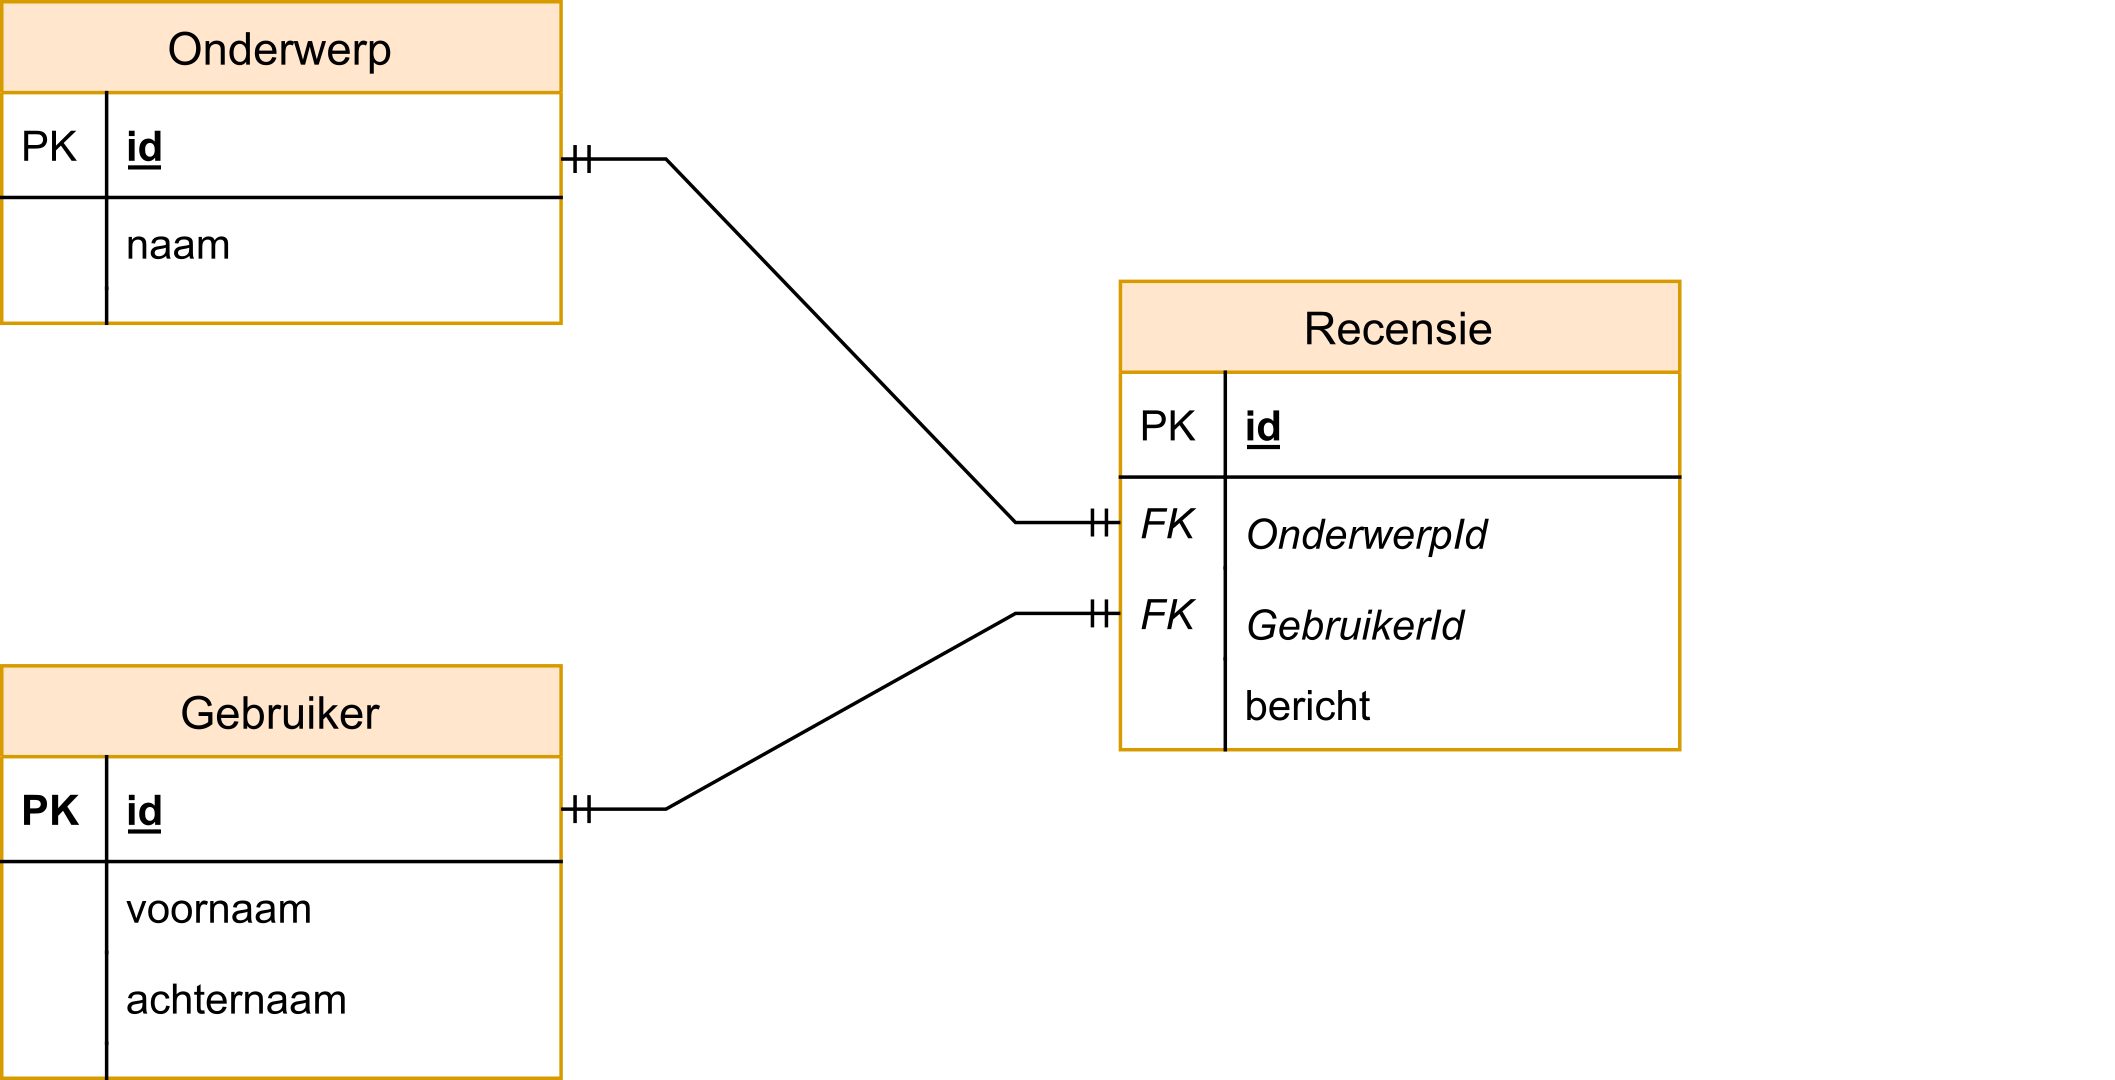
\includegraphics{graphics/erd.png}
  \caption[ERD recensie applicatie]{\label{fig:erd}ERD diagram van de recensie applicatie}
\end{figure}
\begin{listing}[H]
  \centering
  \begin{minted}[bgcolor=bg,
      fontfamily=tt,
      linenos=true,
      numberblanklines=true,
      numbersep=5pt,
      gobble=0,
      framesep=2mm,
      tabsize=4,
      obeytabs=false,
      breaklines=true,
      mathescape=false
      samepage=false,
      showspaces=false,
      showtabs =false,
      texcl=false]{js}
const { Model, DataTypes  } = require("sequelize");

class Gebruiker extends Model {}

async function GebruikerInit(sequelize) {
  Gebruiker.init(
    {
      id: {
        type: DataTypes.INTEGER,
        autoIncrement: true,
        primaryKey: true,
      },
      voornaam: {
        type: DataTypes.STRING,
        allowNull: false,
      },
      achternaam: {
        type: DataTypes.STRING,
      },
    },
    { sequelize, modelName: "Gebruiker" }
  );
  await Gebruiker.sync();
}

module.exports = {
  Gebruiker,
  GebruikerInit,
};
\end{minted}
\caption[Model gebruiker]{\label{code:User}Code van het model van de gebruiker}
\end{listing}

\begin{listing}[H]
  \centering
  \begin{minted}[bgcolor=bg,
      fontfamily=tt,
      linenos=true,
      numberblanklines=true,
      numbersep=5pt,
      gobble=0,
      framesep=2mm,
      tabsize=4,
      obeytabs=false,
      breaklines=true,
      mathescape=false
      samepage=false,
      showspaces=false,
      showtabs =false,
      texcl=false]{js}
const { Model, DataTypes } = require("sequelize");

class Onderwerp extends Model {}

async function OnderwerpInit(sequelize) {
  Onderwerp.init(
    {
      id: {
        type: DataTypes.INTEGER,
        autoIncrement: true,
        primaryKey: true,
      },
      naam: {
        type: DataTypes.STRING,
        allowNull: false,
      },
    },
    { sequelize, modelName: "Onderwerp" }
  );
  await Onderwerp.sync();
}

module.exports = {
  Onderwerp,
  OnderwerpInit,
};
\end{minted}
\caption[Model onderwerp]{\label{code:Subject}Code van het model van het onderwerp}
\end{listing}

\begin{listing}[H]
  \centering
  \begin{minted}[bgcolor=bg,
      fontfamily=tt,
      linenos=true,
      numberblanklines=true,
      numbersep=5pt,
      gobble=0,
      framesep=2mm,
      tabsize=4,
      obeytabs=false,
      breaklines=true,
      mathescape=false
      samepage=false,
      showspaces=false,
      showtabs =false,
      texcl=false]{js}
const { Model, DataTypes } = require("sequelize");
const { Gebruiker } = require("./gebruiker.js");
const { Onderwerp } = require("./onderwerp.js");
class Recensie extends Model {}

module.exports = async (sequelize) => {
  Recensie.init(
    {
      id: {
        type: DataTypes.INTEGER,
        autoIncrement: true,
        primaryKey: true,
      },
      bericht: {
        type: DataTypes.STRING,
        allowNull: false,
      },
    },
    { sequelize, modelName: "Recensie" }
  );
  Recensie.belongsTo(Gebruiker, { onDelete: "CASCADE" });
  Recensie.belongsTo(Onderwerp, { onDelete: "CASCADE" });
  await Recensie.sync();
};
\end{minted}
\caption[Model recensie]{\label{code:Review}Code van het model van de recensie}
\end{listing}

In de code ~\ref{code:Instantie} wordt een connectie aangemaakt met de databank door het gebruik van Sequelize. 
De benodigde configuratie wordt met behulp van de config package opgehaald. Zo is de 
gebruikersnaam, databasenaam, de technologie van de database en het wachtwoord te vinden via de configuratie.
Deze waarden worden via het config package opgehaald uit het environment om zo de veiligheid te waarborgen.
Voor zowel te kunnen werken met MySQL als Postgres wordt gebruikgemaakt van de packages: mysql2 en pg.
Deze configuratie wordt dan gebruikt om de connectie aan te maken en de tabellen te initialiseren.
Nadien  de tabellen voor de gebruiker en de onderwerpen opgevuld met voorbeeldgegevens, zoals weergegeven in ~\ref{code:Seed}.

\begin{listing}[H]
  \centering
  \begin{minted}[bgcolor=bg,
      fontfamily=tt,
      linenos=true,
      numberblanklines=true,
      numbersep=5pt,
      gobble=0,
      framesep=2mm,
      tabsize=4,
      obeytabs=false,
      breaklines=true,
      mathescape=false
      samepage=false,
      showspaces=false,
      showtabs =false,
      texcl=false]{js}
const { Sequelize } = require("sequelize");
const configuration = require("config");
const RecensieMigratie = require("./recensie");
const seed = require("./seeder");
const { GebruikerInit } = require("./gebruiker");
const { OnderwerpInit } = require("./onderwerp");
//config
const username = configuration.get("username");
const database = configuration.get("database");
const dialect = configuration.get("dialect");
const password = configuration.get("password");

// Instantie aanmaken
let sequelize;
async function initializeSequelize() {
  sequelize = new Sequelize(database, username, password, {
    host: dialect,
    dialect: dialect,
    pool: {
      max: 100,
    }
  });
  try {
    await sequelize.authenticate();
    console.log("Connection has been established successfully.");
  } catch (error) {
    console.error("Unable to connect to the database:", error);
  }
  await GebruikerInit(sequelize);
  await OnderwerpInit(sequelize);
  await RecensieMigratie(sequelize);
  await seed(sequelize);
  return sequelize;
}

function getSequelize() {
  if (!sequelize) {
    throw new Error("initialize sequelize");
  }
  return sequelize;
}
module.exports = {
  initializeSequelize,
  getSequelize,
};
\end{minted}
\caption[Sequelize instantie]{\label{code:Instantie}Code bij aanmaken instantie sequelize}
\end{listing}

\begin{listing}[H]
  \centering
  \begin{minted}[bgcolor=bg,
      fontfamily=tt,
      linenos=true,
      numberblanklines=true,
      numbersep=5pt,
      gobble=0,
      framesep=2mm,
      tabsize=4,
      obeytabs=false,
      breaklines=true,
      mathescape=false
      samepage=false,
      showspaces=false,
      showtabs =false,
      texcl=false]{js}
async function seed(sequelize) {
  // Originele staat
  await sequelize.models.Gebruiker.destroy({ truncate: { cascade: true } });
  await sequelize.models.Onderwerp.destroy({ truncate: { cascade: true } });
  await sequelize.models.Gebruiker.create({
    id: 1,
    voornaam: "Quinten",
    achternaam: "De Wolf",
  });
  await sequelize.models.Onderwerp.create({
    id: 1,
    naam: "Auto",
  });
  await sequelize.models.Onderwerp.create({
    id: 2,
    naam: "Vliegtuigen",
  });
  await sequelize.models.Onderwerp.create({
    id: 3,
    naam: "Racing",
  });
}
module.exports = seed;
\end{minted}
\caption[Opvulling tabellen]{\label{code:Seed}Code bij het opvullen van de tabellen}
\end{listing}

Als laatste wordt de server aangemaakt om een POST methode op het recensie endpoint en een GET methode op het onderwerpen endpoint aan te nemen.
In ~\ref{code:NodeServer} wordt de code om dit te bereiken in Node.js getoond. Hierbij komt data in de vorm van JSON binnen voor de POST methode.
Deze bevat de recensie in combinatie met het id van het onderwerp en de gebruiker.
Deze zal dan gebruikt worden om een nieuwe rij aan te maken in de recensie tabel.
Daarnaast is er ook een GET endpoint die de lijst van alle onderwerpen zal ophalen en teruggeven.
In ~\ref{code:BunServer} kan dezelfde functionele code worden gevonden voor Bun.

\begin{listing}[H]
  \centering
  \begin{minted}[bgcolor=bg,
      fontfamily=tt,
      linenos=true,
      numberblanklines=true,
      numbersep=5pt,
      gobble=0,
      framesep=2mm,
      tabsize=4,
      obeytabs=false,
      breaklines=true,
      mathescape=false
      samepage=false,
      showspaces=false,
      showtabs =false,
      texcl=false]{js}
const http = require("node:http");
const { initializeSequelize } = require("./sequelize.js");
async function main() {
  const sequelizeInstance = await initializeSequelize();
  http
    .createServer(async (req, res) => {
      if (req.method === "POST" && req.url === "/recensie") {
        let body = "";
        req.on("data", (data) => {
          body += data.toString(); 
        });
        req.on("end", async () => {
          try {
            const data = JSON.parse(body);
            await sequelizeInstance.models.Recensie.create(data);
            res.writeHead(201, { "Content-Type": "application/json" });
            res.end();
          } catch (error) {
            console.error("Error:", error);
            res.writeHead(400, { "Content-Type": "application/json" });
            res.end(JSON.stringify({ message: "Invalid data" }));
          }
        });
      } else if (req.method === "GET" && req.url === "/onderwerpen") {
        try {
          const data = await sequelizeInstance.models.Onderwerp.findAll();
          res.writeHead(200, { "Content-Type": "application/json" });
          res.end(JSON.stringify(data));
        } catch {
          res.writeHead(500, { "Content-Type": "tet/plain" });
          res.end('Internal Server error')
        }
      }
    })
    .listen(3000);
}
main();
\end{minted}
\caption[Ontvangen van verzoeken in Node.js]{\label{code:NodeServer}Code om de verzoeken te ontvangen binnen Node.js}
\end{listing}
\begin{listing}[H]
  \centering
  \begin{minted}[bgcolor=bg,
      fontfamily=tt,
      linenos=true,
      numberblanklines=true,
      numbersep=5pt,
      gobble=0,
      framesep=2mm,
      tabsize=4,
      obeytabs=false,
      breaklines=true,
      mathescape=false
      samepage=false,
      showspaces=false,
      showtabs =false,
      texcl=false]{js}
const { initializeSequelize } = require("./sequelize.js");
const sequelizeInstance = await initializeSequelize();
Bun.serve({
    port:3000,
    async fetch(request) {
        try {
            const url = new URL(request.url);
            if (request.method === "POST" && url.pathname === "/recensie") {
                const data = await request.json();
                await sequelizeInstance.models.Recensie.create(data);
                return new Response('',{headers: { "Content-Type": "application/json"}, status: 201});
            } else if (request.method === "GET" && url.pathname === "/onderwerpen") {
                const data = await sequelizeInstance.models.Onderwerp.findAll();
                return Response.json(data);
            }
        } catch (error) {
            console.error("Error:", error);
            return new Response(JSON.stringify({ message: 'Invalid data'}), 
            {headers: { "Content-Type": "application/json"}, status: 400})
        }
    }
})
\end{minted}
\caption[Ontvangen van verzoeken in Bun]{\label{code:BunServer}Code om de verzoeken te ontvangen binnen Bun}
\end{listing}
\subsection{Uitvoering metingen}
Voor de metingen worden twee hulpprogramma's gebruikt: Hyperfine en Bombardier.
In \ref{code:HyperfineScript} wordt Hyperfine gebruikt om de gemiddelde uitvoeringstijd over verschillende iteraties van het script te berekenen.
Ook zal Hyperfine gebruikt worden om de gemiddelde installatietijd van de respectievelijke package managers te vergelijken zoals 
te zien is in \ref{code:HyperfineInstall}. Specifiek wordt de installatietijd bekeken wanneer het cache geheugen data bevat.
Bij de metingen wordt telkens versie 1.15 van Hyperfine gebruikt.
\begin{listing}[H]
  \centering
  \begin{minted}[bgcolor=bg,
      fontfamily=tt,
      linenos=true,
      numberblanklines=true,
      numbersep=5pt,  
      gobble=0,
      framesep=2mm,
      tabsize=4,
      obeytabs=false,
      breaklines=true,
      mathescape=false
      samepage=false,
      showspaces=false,
      showtabs =false,
      texcl=false]{shell-session}
> hyperfine --warmup 1 'node index.js 1000' 'bun index.js 1000'
      \end{minted}
      \caption[Gebruik Hyperfine bij het algoritme]{\label{code:HyperfineScript}Gebruik Hyperfine commando bij het algoritme}
\end{listing}

\begin{listing}[H]
  \centering
  \begin{minted}[bgcolor=bg,
      fontfamily=tt,
      linenos=true,
      numberblanklines=true,
      numbersep=5pt,  
      gobble=0,
      framesep=2mm,
      tabsize=4,
      obeytabs=false,
      breaklines=true,
      mathescape=false
      samepage=false,
      showspaces=false,
      showtabs =false,
      texcl=false]{shell-session}
> hyperfine --prepare 'rm -rf node_modules' --warmup 1 --runs 100 'npm install' 'bun install'
      \end{minted}
      \caption[Gebruik Hyperfine bij de installatie]{\label{code:HyperfineInstall}Gebruik Hyperfine commando bij de installtie}
\end{listing}
Daarnaast wordt voor de HTTP server gebruikgemaakt van Bombardier. 
Hierbij kan ingesteld worden hoeveel gelijktijdige connecties er zijn en hoeveel verzoeken per test worden verstuurd.
In de metingen worden 500000 verzoeken verzonden met 10, 50 en 100 gelijktijdige verbindingen.
De commando's hiervoor staan vermeld in \ref{code:Bombardier10}, \ref{code:Bombardier100} en \ref{code:Bombardier1000}.
Hierbij wordt telkens een POST verzoek gestuurd. In \ref{code:Bombardier10GET} wordt een voorbeeld getoond om GET verzoeken te sturen.
Voor deze metingen wordt versie 1.2.6 van Bombardier gebruikt.
\begin{listing}[H]
  \centering
  \begin{minted}[bgcolor=bg,
      fontfamily=tt,
      linenos=true,
      numberblanklines=true,
      numbersep=5pt,  
      gobble=0,
      framesep=2mm,
      tabsize=4,
      obeytabs=false,
      breaklines=true,
      mathescape=false
      samepage=false,
      showspaces=false,
      showtabs =false,
      texcl=false]{shell-session}
> bombardier -c 10 -n 500000 -m POST -b '{"bericht": "test","GebruikerId": 1,"OnderwerpId": 1}' -l http://localhost:3000/recensie
      \end{minted}
      \caption[Gebruik Bombardier POST verzoek met 10 connecties]{\label{code:Bombardier10}Gebruik Bombardier commando met 500000 verzoeken en 10 gelijktijdige connecties voor een POST verzoek}
\end{listing}
\begin{listing}[H]
  \centering
  \begin{minted}[bgcolor=bg,
      fontfamily=tt,
      linenos=true,
      numberblanklines=true,
      numbersep=5pt,  
      gobble=0,
      framesep=2mm,
      tabsize=4,
      obeytabs=false,
      breaklines=true,
      mathescape=false
      samepage=false,
      showspaces=false,
      showtabs =false,
      texcl=false]{shell-session}
> bombardier -c 50 -n 500000 -m POST -b '{"bericht": "test","GebruikerId": 1,"OnderwerpId": 1}' -l http://localhost:3000/recensie
      \end{minted}
      \caption[Gebruik Bombardier POST verzoek met 50 connecties]{\label{code:Bombardier100}Gebruik Bombardier commando met 500000 verzoeken en 50 gelijktijdige connecties voor een POST verzoek}
\end{listing}
\begin{listing}[H]
  \centering
  \begin{minted}[bgcolor=bg,
      fontfamily=tt,
      linenos=true,
      numberblanklines=true,
      numbersep=5pt,  
      gobble=0,
      framesep=2mm,
      tabsize=4,
      obeytabs=false,
      breaklines=true,
      mathescape=false
      samepage=false,
      showspaces=false,
      showtabs =false,
      texcl=false]{shell-session}
> bombardier -c 100 -n 500000 -m POST -b '{"bericht": "test","GebruikerId": 1,"OnderwerpId": 1}' -l http://localhost:3000/recensie
      \end{minted}
      \caption[Gebruik Bombardier POST verzoek met 100 connecties]{\label{code:Bombardier1000}Gebruik Bombardier commando met 500000 verzoeken en 100 gelijktijdige connecties voor een POST verzoek}
\end{listing}
\begin{listing}[H]
  \centering
  \begin{minted}[bgcolor=bg,
      fontfamily=tt,
      linenos=true,
      numberblanklines=true,
      numbersep=5pt,  
      gobble=0,
      framesep=2mm,
      tabsize=4,
      obeytabs=false,
      breaklines=true,
      mathescape=false
      samepage=false,
      showspaces=false,
      showtabs =false,
      texcl=false]{shell-session}
> bombardier -c 10 -n 500000 -l http://localhost:3000/onderwerpen
      \end{minted}
      \caption[Gebruik Bombardier GET verzoek 10 connecties]{\label{code:Bombardier10GET}Gebruik Bombardier commando met 500000 verzoeken en 10 gelijktijdige connecties voor een GET verzoek}
\end{listing}
Bij de uitvoering wordt gewerkt met een vorm van containervirtualisatie genaamd Docker.
Hierbij zit elke applicatie in zijn eigen container waarbij aan de hand van een Dockerfile deze telkens wordt opgezet.
In \ref{code:dockerscript} is de Dockerfile voor het QuickSort algoritme te zien. 
Hierbij wordt vertrokken van een omgeving die Node.js al bevat waar nadien Hyperfine en Bun worden geïnstalleerd.
Hierna wordt dan met behulp van Hyperfine de uitvoeringstijd van Bun en Node.js berekend.
Dit bestand moet eerst gebouwd worden met het “docker build” commando waarvan een voorbeeld te vinden is in \ref{code:dockerbuild}.
Daarna moet de image worden uitgevoerd met het “docker run” commando zoals het voorbeeld in \ref{code:dockerrun}.
Voor de HTTP server is er nog een bijkomend
Docker Compose bestand waar aan de hand van het commando in \ref{code:dockercompose}
zowel de databank als de server kan worden opgestart. Een voorbeeld hiervan voor zowel een MySQL database als een PostgreSQL database is 
respectievelijk te vinden in \ref{code:dockercomposefile} en \ref{code:dockercomposepostgres}.
Hierbij wordt dan ook een Dockerfile gebruikt om de server te starten. De Dockerfile voor de Node.js en Bun server 
zijn respectievelijk te vinden in \ref{code:dockernode} en \ref{code:dockerbun}. 
Om het gemiddelde CPU-gebruik en het maximale geheugengebruik te bepalen wordt Bombardier samen met het “docker stats” commando uitgevoerd in een zsh script.
Hierbij wordt vóór het uitvoeren van Bombardier de monitoring gestart van het geheugen- en CPU-gebruik. 
Na de uitvoering wordt het gemiddelde CPU-gebruik en het maximale geheugengebruik bepaald.
Een voorbeeld van dit script is te vinden in \ref{code:zshscript}. 
In dit voorbeeld wordt zowel de Bombardier om de POST methode als de GET methode weergegeven. Afhankelijk van wat gemeten wordt, moet tussen 1 van deze 2 methoden gekozen worden.
Het aantal connecties kan als argument meegegeven worden bij de uitvoering van het script.
Bij de server wordt ook de installatietijd van de package managers gemeten met behulp van de Dockerfile \ref{code:dockerinstall}.
Hiervoor wordt ook Hyperfine gebruikt, waarbij de cache al wordt opgevuld door de “warmup” in het commando.
Tot slot wordt voor het maximale geheugengebruik bij het script het zsh time commando gebruikt. Hierbij wordt de omgevingsvariabele 
ingesteld zodat het maximaal geheugengebruik kan getoond worden zoals in \ref{code:zshmemory}
\begin{listing}[H]
  \centering
  \begin{minted}[bgcolor=bg,
      fontfamily=tt,
      linenos=true,
      numberblanklines=true,
      numbersep=5pt,  
      gobble=0,
      framesep=2mm,
      tabsize=4,
      obeytabs=false,
      breaklines=true,
      mathescape=false
      samepage=false,
      showspaces=false,
      showtabs =false,
      texcl=false]{bash}
# Base image met Node.js geïnstalleerd
FROM node:21

# Installeer Hyperfine met apt
RUN apt-get update && \
    apt-get install -y curl && \
    apt-get install -y hyperfine=1.15.0-2
# Zet de werk map in de container
WORKDIR /app

# Download bun
RUN curl -fsSL https://bun.sh/install | bash -s "bun-v1.1.3" && \
  ln -s $HOME/.bun/bin/bun /usr/local/bin/bun

# Kopieer de applicatie code naar de container
COPY . .
RUN ~/.bun/bin/bun install
# Commando dat wordt uitgevoerd wanneer container start
CMD ["hyperfine","--warmup", "1", "node index.js 1000", "bun index.js 1000"]
      \end{minted}
      \caption[Dockerfile QuickSort algoritme]{\label{code:dockerscript}Dockerfile voor het QuickSort algoritme}
\end{listing}
\begin{listing}[H]
  \centering
  \begin{minted}[bgcolor=bg,
      fontfamily=tt,
      linenos=true,
      numberblanklines=true,
      numbersep=5pt,  
      gobble=0,
      framesep=2mm,
      tabsize=4,
      obeytabs=false,
      breaklines=true,
      mathescape=false
      samepage=false,
      showspaces=false,
      showtabs =false,
      texcl=false]{shell-session}
> docker build -f "Dockerfile" -t testimage .
      \end{minted}
      \caption[Commando voor docker image te bouwen]{\label{code:dockerbuild}Voorbeeld bouwen van een Docker image met naam testimage}
\end{listing}
\begin{listing}[H]
  \centering
  \begin{minted}[bgcolor=bg,
      fontfamily=tt,
      linenos=true,
      numberblanklines=true,
      numbersep=5pt,  
      gobble=0,
      framesep=2mm,
      tabsize=4,
      obeytabs=false,
      breaklines=true,
      mathescape=false
      samepage=false,
      showspaces=false,
      showtabs =false,
      texcl=false]{shell-session}
> docker run -it testimage .
      \end{minted}
      \caption[Commando voor Docker image uit te voeren]{\label{code:dockerrun}Voorbeeld uitvoeren van een Docker image met naam testimage}
\end{listing}

\begin{listing}[H]
  \centering
  \begin{minted}[bgcolor=bg,
      fontfamily=tt,
      linenos=true,
      numberblanklines=true,
      numbersep=5pt,  
      gobble=0,
      framesep=2mm,
      tabsize=4,
      obeytabs=false,
      breaklines=true,
      mathescape=false
      samepage=false,
      showspaces=false,
      showtabs =false,
      texcl=false]{shell-session}
> docker-compose -f docker-compose.yml up --build
      \end{minted}
      \caption[Uitvoering Docker Compose]{\label{code:dockercompose}Uitvoeren van een Docker Compose bestand}
\end{listing}
\begin{listing}[H]
  \centering
  \begin{minted}[bgcolor=bg,
      fontfamily=tt,
      linenos=true,
      numberblanklines=true,
      numbersep=5pt,  
      gobble=0,
      framesep=2mm,
      tabsize=4,
      obeytabs=false,
      breaklines=true,
      mathescape=false
      samepage=false,
      showspaces=false,
      showtabs =false,
      texcl=false]{yaml}
version: '3'

services:
  mysql:
    image: mysql:latest
    environment:
      MYSQL_ROOT_PASSWORD: Test12345
      MYSQL_DATABASE: review
    ports:
      - "3306:3306"
    healthcheck:
      test: ["CMD", "mysqladmin", "ping", "-h", "localhost"]
      interval: 5s
      timeout: 3s
      retries: 5

  bun:
    build: .
    depends_on:
      mysql:
        condition: service_healthy
    ports:
      - "3000:3000"
    environment:
      DB_PORT: 3306
      DB_USER: root
      DB_PASSWORD: Test12345
      DB_DATABASE: review
      DB_DIALECT: mysql
      \end{minted}
      \caption[Docker Compose bestand voor MySQL]{\label{code:dockercomposefile}Docker Compose bestand voor het opstarten van de MySQL database en server}
\end{listing}
\begin{listing}[H]
  \centering
  \begin{minted}[bgcolor=bg,
      fontfamily=tt,
      linenos=true,
      numberblanklines=true,
      numbersep=5pt,  
      gobble=0,
      framesep=2mm,
      tabsize=4,
      obeytabs=false,
      breaklines=true,
      mathescape=false
      samepage=false,
      showspaces=false,
      showtabs =false,
      texcl=false]{yaml}
version: '3'

services:
  postgres:
    image: postgres:latest
    environment:
      POSTGRES_PASSWORD: Test12345
      POSTGRES_DB: review
      PGDATA: /data/postgres
    ports:
      - "5432:5432"
    healthcheck:
      test: ["CMD-SHELL", "pg_isready -U postgres"]
      interval: 5s
      timeout: 3s
      retries: 5

  bun:
    build: .
    depends_on:
      postgres:
        condition: service_healthy
    ports:
      - "3000:3000"
    environment:
      DB_PORT: 5432
      DB_USER: postgres
      DB_PASSWORD: Test12345
      DB_DATABASE: review
      DB_DIALECT: postgres
      \end{minted}
      \caption[Docker Compose bestand voor PostgreSQL]{\label{code:dockercomposepostgres}Docker Compose bestand voor het opstarten van de PostgreSQL database en server}
\end{listing}
\begin{listing}[H]
  \centering
  \begin{minted}[bgcolor=bg,
      fontfamily=tt,
      linenos=true,
      numberblanklines=true,
      numbersep=5pt,  
      gobble=0,
      framesep=2mm,
      tabsize=4,
      obeytabs=false,
      breaklines=true,
      mathescape=false
      samepage=false,
      showspaces=false,
      showtabs =false,
      texcl=false]{bash}
# Base image met Node.js geïnstalleerd
FROM node:21

# Zet de werk map in de container
WORKDIR /app

# Kopieer de package.json and package-lock.json bestanden naar de container
COPY package*.json ./

# Installeer dependencies
RUN npm install

# Kopieer de rest van de applicatie code naar de container
COPY . .

# Zet de poort open
EXPOSE 3000

# Commando dat wordt uitgevoerd wanneer container start
CMD ["npm", "run", "dev"]
      \end{minted}
      \caption[Dockerfile Node.js server]{\label{code:dockernode}Dockerfile voor de Node.js server}
\end{listing}


\begin{listing}[H]
  \centering
  \begin{minted}[bgcolor=bg,
      fontfamily=tt,
      linenos=true,
      numberblanklines=true,
      numbersep=5pt,  
      gobble=0,
      framesep=2mm,
      tabsize=4,
      obeytabs=false,
      breaklines=true,
      mathescape=false
      samepage=false,
      showspaces=false,
      showtabs =false,
      texcl=false]{bash}
# Base image met bun geïnstalleerd
FROM oven/bun:1.1.3 as base

# Zet de werk map in de container
WORKDIR /usr/src/app

# Kopieer de package.json and package-lock.json bestanden naar de container
COPY package.json bun.lockb ./
# Installeer dependencies
RUN bun install

# Kopieer de rest van de applicatie code naar de container
COPY . .

# Zet de poort open
EXPOSE 3000

# Commando dat wordt uitgevoerd wanneer container start
CMD ["bun", "run", "index.js"]
      \end{minted}
      \caption[Dockerfile Bun server]{\label{code:dockerbun}Dockerfile voor de Bun server}
\end{listing}

\begin{listing}[H]
  \centering
  \begin{minted}[bgcolor=bg,
      fontfamily=tt,
      linenos=true,
      numberblanklines=true,
      numbersep=5pt,  
      gobble=0,
      framesep=2mm,
      tabsize=4,
      obeytabs=false,
      breaklines=true,
      mathescape=false
      samepage=false,
      showspaces=false,
      showtabs =false,
      texcl=false]{bash}
#!/bin/zsh

# Start de monitoring
docker stats <container_naam> --format "table {{.Container}}\t{{.CPUPerc}}\t{{.MemUsage}}" > container_stats.txt &

# Start bombardier POST
bombardier -c "$1" -n 500000 -m POST -b '{"bericht": "test","GebruikerId": 1,"OnderwerpId": 1}' -l http://localhost:3000/recensie
# Of
# Start bombardier GET
bombardier -c "$1" -n 500000 -l http://localhost:3000/onderwerpen

# Stop de docker stats

target_command="/Applications/Docker.app/Contents/Resources
/bin/com.docker.cli stats"
docker_cli_pid=$(ps aux | grep "$target_command" | grep -v grep | awk '{print $2}')

if [[ -n $docker_cli_pid ]]; then
    echo "Killing Docker CLI process with PID: $docker_cli_pid"
    kill -9 $docker_cli_pid
else
    echo "Docker CLI process not found."
fi

# Bereken gemiddeld CPU-gebruik en hoogste memory
while IFS= read -r line; do
    if [[ $line =~ ([0-9]+\.[0-9]+)%(.*[0-9]+\.[0-9]+)MiB ]]; then
        cpu_percent="${match[1]}"
        mem_usage="${match[2]}"
        cpu_percent_sum=$((cpu_percent_sum + cpu_percent))
        if (( mem_usage > highest_mem_usage )); then
            highest_mem_usage="$mem_usage"
        fi
        ((total_lines++))
    fi
done < container_stats.txt

average_cpu_percent=$((cpu_percent_sum / total_lines))
# Toon resultaten
echo "Gemiddelde CPU-gebruik: $average_cpu_percent%"
echo "Maximaal geheugen gebruik: $highest_mem_usage"
      \end{minted}
      \caption[Dockerfile QuickSort algoritme]{\label{code:zshscript}Dockerfile voor het QuickSort algoritme}
\end{listing}

\begin{listing}[H]
  \centering
  \begin{minted}[bgcolor=bg,
      fontfamily=tt,
      linenos=true,
      numberblanklines=true,
      numbersep=5pt,  
      gobble=0,
      framesep=2mm,
      tabsize=4,
      obeytabs=false,
      breaklines=true,
      mathescape=false
      samepage=false,
      showspaces=false,
      showtabs =false,
      texcl=false]{bash}
# Base image met Node.js geïnstalleerd
FROM node:21

# Installeer Hyperfine met apt
RUN apt-get update && \
    apt-get install -y curl && \
    apt-get install -y hyperfine=1.15.0-2
# Zet de werk map in de container
WORKDIR /app

RUN curl -fsSL https://bun.sh/install | bash -s "bun-v1.1.3" && \
  ln -s $HOME/.bun/bin/bun /usr/local/bin/bun

# Kopieer de applicatiebestanden naar de container
COPY . .
RUN ~/.bun/bin/bun install
# Commando dat wordt uitgevoerd wanneer container start
CMD ["hyperfine","--prepare", "rm -rf node_modules", "--warmup","1","--runs","100","bun install","npm install"]
      \end{minted}
      \caption[Dockerfile meting installatietijd]{\label{code:dockerinstall}Dockerfile voor de installatietijd te meten bij de server}
\end{listing}

\begin{listing}[H]
  \centering
  \begin{minted}[bgcolor=bg,
      fontfamily=tt,
      linenos=true,
      numberblanklines=true,
      numbersep=5pt,  
      gobble=0,
      framesep=2mm,
      tabsize=4,
      obeytabs=false,
      breaklines=true,
      mathescape=false
      samepage=false,
      showspaces=false,
      showtabs =false,
      texcl=false]{shell-session}
> TIMEFMT='%J   %U  user %S system %P cpu %*E total'$'\n'\
'max memory:                %M '$MAX_MEMORY_UNITS''$'\n'\
> time node index.js 1000
> time bun index.js 1000
      \end{minted}
      \caption[Dockerfile time commando]{\label{code:zshmemory}Aanpassing zsh commando voor maximaal geheugengebruik te tonen}
\end{listing}

\subsection{Resultaten proof-of-concept}
In deze sectie zullen de resultaten van de performantie testen besproken worden.
Hierbij worden eerst de resultaten voor de uitvoeringstijd bij het QuickSort algoritme bekeken.
Vervolgens worden de resultaten van de server besproken op het gebied van uitvoeringstijd, CPU-gebruik, geheugengebruik, latentie en de installatietijd
zowel bij het gebruik van een MySQL database als een PostgreSQL database.

\subsubsection{Resultaten  QuickSort algoritme}
De resultaten voor de gemiddelde uitvoeringstijd bij het QuickSort algoritme werden bekomen met behulp van Hyperfine.
Hierbij werd gekeken naar de uitvoeringstijd voor het sorteren van een array bestaande uit 1000 elementen met volgende commando \ref{code:HyperfineScript}.
Bun heeft hierbij een gemiddelde uitvoeringstijd van 6.4 milliseconden met een standaardafwijking van 0.8 milliseconden. 
Dit tegenover de gemiddelde uitvoeringstijd van 14.1 milliseconden bij Node.js met een standaardafwijking van 1.3 milliseconden.
In figuur \ref{fig:uitvoeringstijdscript} wordt de gemiddelde uitvoeringstijd per omgeving visueel voorgesteld
Daarbij is op te merken dat de gemiddelde uitvoeringstijd van Bun 2.21 keer sneller is dan bij Node.js.
In figuur \ref{fig:RAMscript} wordt het maximale geheugengebruik voor zowel Bun als Node.js weergegeven. 
Hierbij werd het time commando telkens 5 keer uitgevoerd.
De resultaten tonen aan dat Bun met 30.69 MB een lager geheugengebruik heeft dan Node.js met 36.4 MB.
\begin{figure}[H]
  \centering
  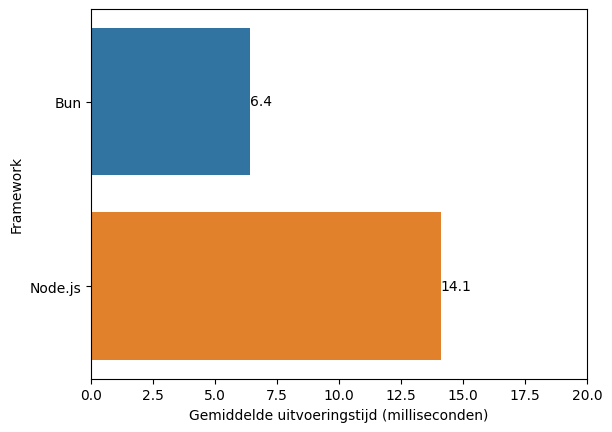
\includegraphics{graphics/scriptuitvoeringstijd.png}
  \caption[Uitvoeringstijd QuickSort algoritme]{\label{fig:uitvoeringstijdscript}Gemiddelde uitvoeringstijd van het QuickSort algoritme voor Bun en Node.js}
\end{figure}

\begin{figure}[H]
  \centering
  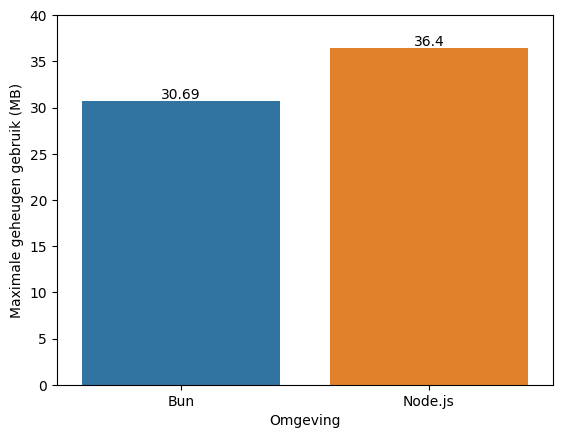
\includegraphics{graphics/RAMScript.png}
  \caption[Geheugengebruik QuickSort algoritme]{\label{fig:RAMscript}Maximale geheugengebruik van het QuickSort algoritme voor Bun en Node.js}
\end{figure}

\subsection{Resultaten Recensie applicatie}
De resultaten voor de gemiddelde installatietijd bij de package managers werden bekomen met behulp van Hyperfine.
Hierbij werd eerst een warmup uitvoering gedaan om de cache al op te vullen.
In figuur \ref{fig:installatietijdapp} zijn de resultaten visueel voorgesteld per omgeving.
Hierbij is op te merken dat Bun met een gemiddelde installatietijd van 24,9 milliseconden en een standaardafwijking van 2,4 milliseconden 24,5 keer sneller 
is dan Node.js, met een gemiddelde installatietijd van 610,1 milliseconden en een standaardafwijking van 100,1 milliseconden.
Voor de overige metingen werd gebruikgemaakt van Bombardier,waarbij
telkens 500.000 verzoeken naar de server werden gestuurd met 10, 50 en 100 gelijktijdige verbindingen.
\begin{figure}[H]
  \centering
  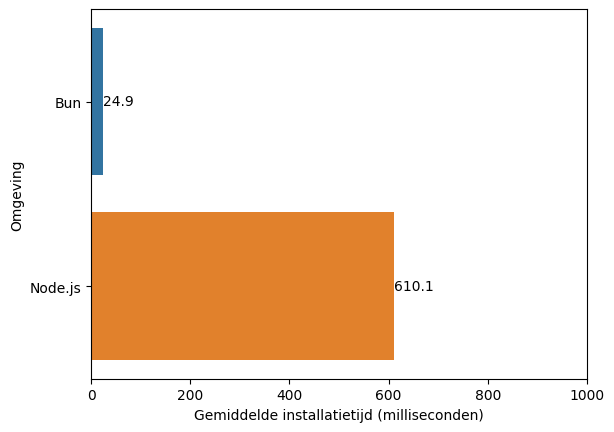
\includegraphics{graphics/install.png}
  \caption[Gemiddelde Installatietijd]{\label{fig:installatietijdapp}Gemiddelde installatietijd van de packages in Bun en Node.js}
\end{figure}



\subsubsection{Resultaten voor de applicatie met een MySQL database}
In deze sectie worden de bekomen resultaten van de applicatie besproken waarbij een MySQL database werd gebruikt.
In tabel \ref{tab:getbombardier} kunnen de resultaten gezien worden van de metingen waarbij de onderwerpen werden opgehaald aan de hand van een GET verzoek.
Er wordt gestreefd naar een zo hoog mogelijk aantal verzoeken per seconde met een zo laag mogelijke latentie, geheugengebruik en CPU-gebruik.
Zoals te zien scoort Bun op het vlak van aantal verzoeken per seconde en latentie beter dan Node.js ongeacht van het aantal connecties. 
Echter heeft Bun bij het aantal verzoeken per seconde wel telkens een grotere standaardafwijking en zijn er dus meer uitschieters aanwezig zijn.
Langs de andere kant verbruikt Bun meer middelen. Zo heeft Bun telkens een hoger CPU-gebruik en zijn de pieken van het geheugen consistent hoger dan bij Node.js.
In figuren \ref{fig:getaantalverzoekenmysql}, \ref{fig:getaantallatentienmysql}, \ref{fig:getgeheugenmysql} en \ref{fig:getcpumysql} kunnen de visuele voorstellingen 
voor respectievelijk het aantal verzoeken per seconde, het aantal latentie, het maximale geheugengebruik en het gemiddelde CPU-gebruik worden gevonden.
\begin{table}[]
  \tabcolsep=0.13cm
  \begin{tabular}{|c|cccccc|}
  \hline
  \multicolumn{1}{|l|}{}                                                                     & \multicolumn{1}{l}{} & Bun      & \multicolumn{1}{l|}{}    & \multicolumn{1}{l}{} & \multicolumn{1}{l}{Node.js} & \multicolumn{1}{l|}{} \\ \hline
  Aantal connecties                                                                          & 10                   & 50       & \multicolumn{1}{c|}{100} & 10                   & 50                          & 100                   \\ \hline
  \begin{tabular}[c]{@{}c@{}}Gemiddeld aantal \\ verzoeken per seconde\end{tabular}          & 9069.30              & 10489.67 & 9298.56                  & 7314.91              & 8985.16                     & 8500.49               \\ \cline{1-1}
  \begin{tabular}[c]{@{}c@{}}Standaardafwijking aantal \\ verzoeken per seconde\end{tabular} & 2974.14              & 3398.39  & 3063.49                  & 2930.06              & 2813.57                     & 2759.61               \\ \cline{1-1}
  \begin{tabular}[c]{@{}c@{}}Latentie \\ (milliseconden)\end{tabular}                        & 1.10                 & 4.76     & 10.76                    & 1.31                 & 5.56                        & 11.77                 \\ \cline{1-1}
  \begin{tabular}[c]{@{}c@{}}Standaardafwijking\\ latentie\\ (milliseconden)\end{tabular}    & 0.72090              & 1.94     & 3.17                     & 1.15                 & 1.63                        & 2.78                  \\ \cline{1-1}
  \begin{tabular}[c]{@{}c@{}}Maximale \\ geheugengebruik \\ (MB)\end{tabular}                & 110.7                & 175.7    & 261.7                    & 104.4                & 114.8                       & 133.3                 \\ \cline{1-1}
  \begin{tabular}[c]{@{}c@{}}Gemiddeld\\ CPU-gebruik\\ (\%)\end{tabular}                     & 110.4                & 112.25   & 116.09                   & 95.24                & 101.64                      & 102.7                 \\ \hline
  \end{tabular}
  \caption[Resultaten GET verzoek met MySQL]{\label{tab:getbombardier}Resultaten metingen waarbij onderwerpen worden opgehaald met een GET verzoek uit de MySQL database.}
  \end{table}

  \begin{figure}[H]
    \centering
    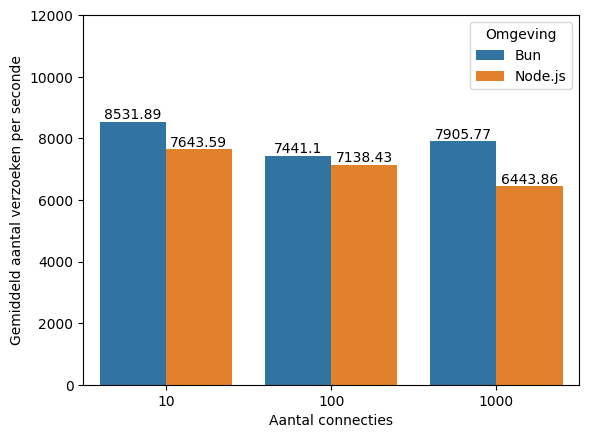
\includegraphics[width=0.7\columnwidth]{graphics/GetMySqlVerzoeken.png}
    \caption[Aantal verzoeken per seconde GET verzoek met MySQL]{\label{fig:getaantalverzoekenmysql}Visuele voorstelling gemiddeld aantal verzoeken per seconde bij het ophalen van de onderwerpen met MySQL.}
  \end{figure}
  \begin{figure}[H]
    \centering
    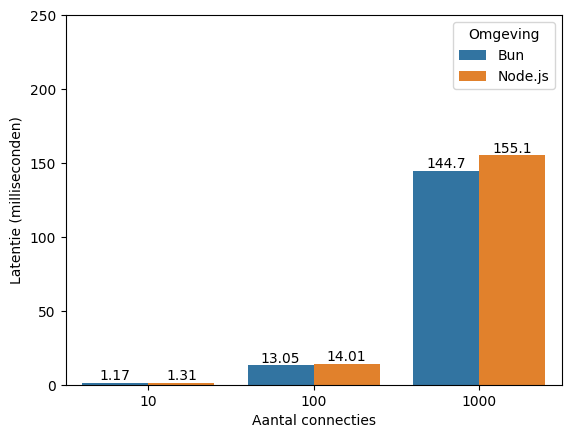
\includegraphics[width=0.7\columnwidth]{graphics/GetMySqlLatentie.png}
    \caption[Latentie GET verzoek met MySQL]{\label{fig:getaantallatentienmysql}Visuele voorstelling gemiddelde latentie bij het ophalen van de onderwerpen met MySQL.}
  \end{figure}
  \begin{figure}[H]
    \centering
    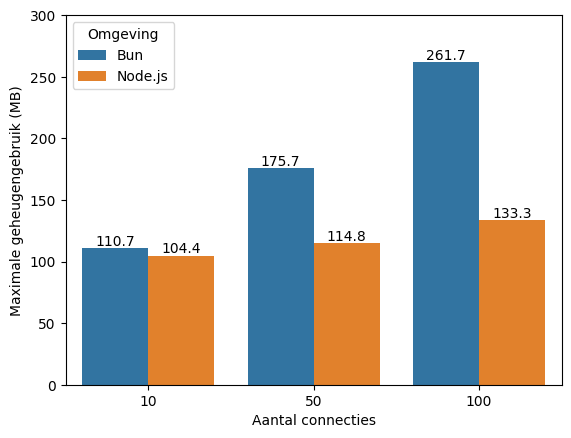
\includegraphics[width=0.7\columnwidth]{graphics/GetMySqlRAM.png}
    \caption[Geheugengebruik GET verzoek met MySQL]{\label{fig:getgeheugenmysql}Visuele voorstelling maximale geheugengebruik bij het ophalen van de onderwerpen met MySQL.}
  \end{figure}
  \begin{figure}[H]
    \centering
    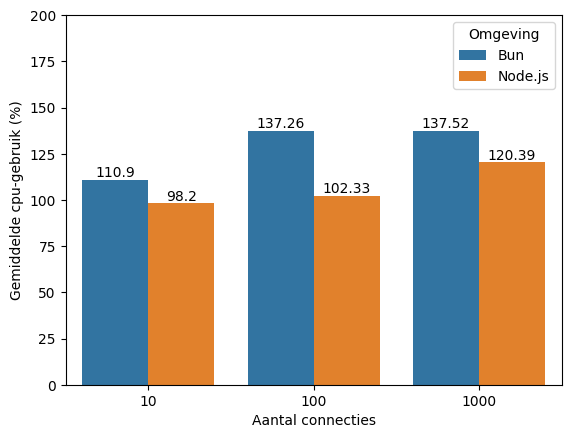
\includegraphics[width=0.7\columnwidth]{graphics/GetMySqlCpu.png}
    \caption[CPU-gebruik GET verzoek met MySQL]{\label{fig:getcpumysql}Visuele voorstelling gemiddeld CPU-gebruik bij het ophalen van de onderwerpen met MySQL.}
  \end{figure}

In tabel \ref{tab:postbombardier} kunnen de resultaten worden bekeken van de metingen waarbij 
een gebruiker een recensie schrijft over een bepaald onderwerp door middel van een POST verzoek.
Hierbij is op te merken dat Bun op zowel bij het gemiddeld aantal verzoeken als latentie gelijkaardig scoort aan Node.js bij 10 connecties. Zo heeft Bun
een gemiddeld aantal verzoeken van 4483 terwijl Node.js hierbij een gemiddelde heeft van 4504.87 heeft. 
Ook bij de latentie is dit het geval waarbij Bun een latentie heeft van 2.27 milliseconden en Node.js een latentie van 2.22 milliseconden.
Deze trend zet zich echter niet voort bij de 50 en 100 connecties waarbij Bun steeds beter presteert op vlak van latentie en aantal verzoeken per seconde.
Node.js heeft bij latentie ook een substantieel grotere standaardafwijking die merkbaar is bij 100 gelijktijdige connecties.
Echter zit er wel consistentie bij het geheugengebruik tussen het aantal connecties.
Bij 10 connecties heeft Bun al een geheugengebruik van 161.2MB terwijl Node.js hier maar een verbruik heeft van 138.2MB.
Voor de 50 en 100 connecties zit Bun telkens hoger dan Node.js.
Hetzelfde is te zien bij het gemiddeld CPU-gebruik voor de 50 en 100 connecties, waarbij Bun respectievelijk
een gemiddeld verbruik van 109.43\% en 118.56\% heeft tegenover Node.js met een gemiddelde van 98.4\% en 107.73\% heeft.
In figuren \ref{fig:postaantalverzoekenmysql}, \ref{fig:postaantallatentienmysql}, \ref{fig:postgeheugenmysql} en \ref{fig:postcpumysql} kunnen de visuele voorstellingen 
voor respectievelijk het aantal verzoeken per seconde, het aantal latentie, het maximale geheugengebruik en het gemiddeld CPU-gebruik worden gevonden.
\begin{table}[H]
  \tabcolsep=0.13cm
  \begin{tabular}{|c|cccccc|}
  \hline
  \multicolumn{1}{|l|}{}                                                                     & \multicolumn{1}{l}{} & Bun     & \multicolumn{1}{l|}{}    & \multicolumn{1}{l}{} & \multicolumn{1}{l}{Node.js} & \multicolumn{1}{l|}{} \\ \hline
  Aantal connecties                                                                          & 10                   & 50      & \multicolumn{1}{c|}{100} & 10                   & 50                          & 100                   \\ \hline
  \begin{tabular}[c]{@{}c@{}}Gemiddeld aantal \\ verzoeken per seconde\end{tabular}          & 4483                 & 5856.48 & 5902.12                  & 4504.87              & 5498.57                     & 5282.67               \\ \cline{1-1}
  \begin{tabular}[c]{@{}c@{}}Standaardafwijking aantal \\ verzoeken per seconde\end{tabular} & 904.95               & 2006.84 & 2204.15                  & 981.92               & 2032.85                     & 2226.43               \\ \cline{1-1}
  \begin{tabular}[c]{@{}c@{}}Latentie \\ (milliseconden)\end{tabular}                        & 2.27                 & 8.54    & 16.95                    & 2.22                 & 9.10                        & 18.94                 \\ \cline{1-1}
  \begin{tabular}[c]{@{}c@{}}Standaardafwijking\\ latentie\\ (milliseconden)\end{tabular}    & 1.17                 & 2.75    & 4.63                     & 1.10                 & 3.46                        & 16.81                 \\ \cline{1-1}
  \begin{tabular}[c]{@{}c@{}}Maximale \\ geheugengebruik \\ (MB)\end{tabular}                & 161.2                & 196.4   & 238.8                    & 138.2                & 115.85                      & 174.6                 \\ \cline{1-1}
  \begin{tabular}[c]{@{}c@{}}Gemiddeld\\ CPU-gebruik\\ (\%)\end{tabular}                     & 63.30                & 109.43  & 118.56                   & 66.26                & 98.4                        & 107.73                \\ \hline
  \end{tabular}
  \caption[Resultaten POST verzoek met MySQL]{\label{tab:postbombardier}Resultaten metingen waarbij door een bepaalde gebruiker een recensie over een onderwerp werd gemaakt in de MySQL database met een POST verzoek.}
  \end{table}
    \begin{figure}[H]
      \centering
      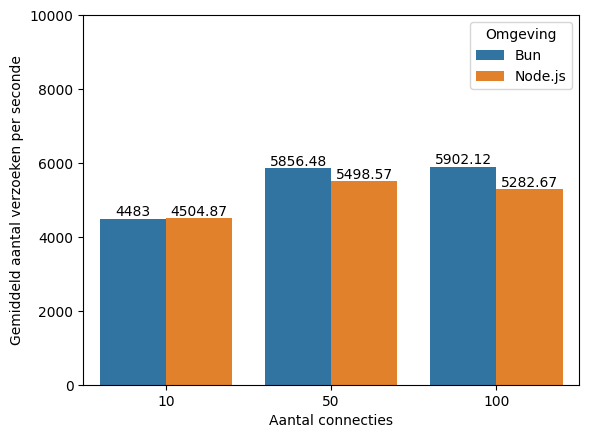
\includegraphics[width=0.7\columnwidth]{graphics/PostMySqlVerzoeken.png}
      \caption[Aantal verzoeken per seconde POST verzoek met MySQL]{\label{fig:postaantalverzoekenmysql}Visuele voorstelling gemiddeld aantal verzoeken per seconde bij het maken van een recensie met MySQL.}
    \end{figure}
    \begin{figure}[H]
      \centering
      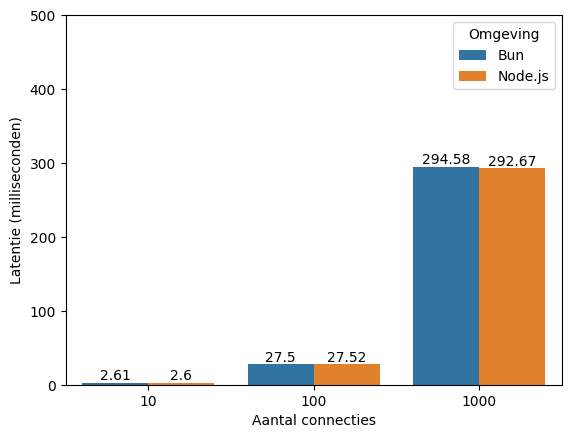
\includegraphics[width=0.7\columnwidth]{graphics/PostMySqlLatentie.png}
      \caption[Latentie POST verzoek met MySQL]{\label{fig:postaantallatentienmysql}Visuele voorstelling gemiddelde latentie bij het maken van een recensie met MySQL.}
    \end{figure}
    \begin{figure}[H]
      \centering
      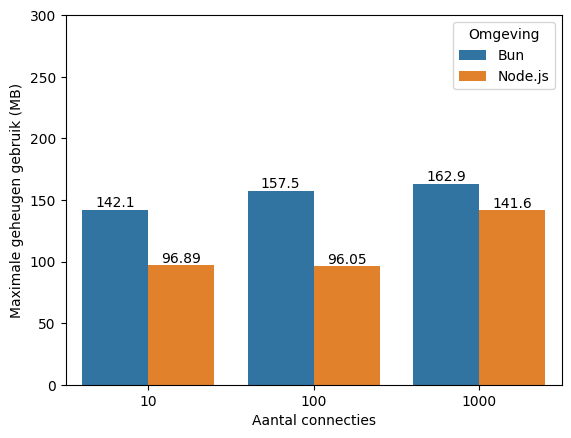
\includegraphics[width=0.7\columnwidth]{graphics/PostMySqlRAM.png}
      \caption[Geheugengebruik POST verzoek met MySQL]{\label{fig:postgeheugenmysql}Visuele voorstelling maximale geheugen gebruik bij het maken van een recensie met MySQL.}
    \end{figure}
    \begin{figure}[H]
      \centering
      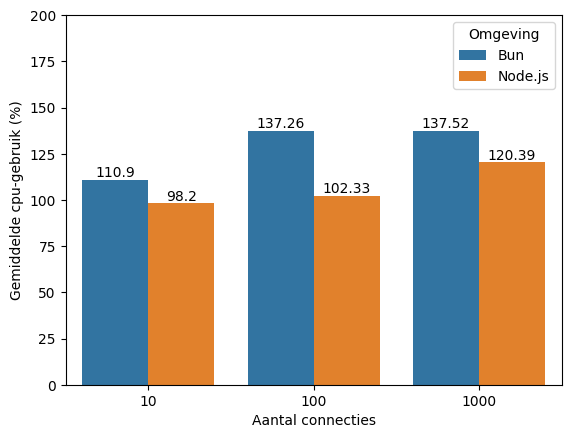
\includegraphics[width=0.7\columnwidth]{graphics/PostMySqlCpu.png}
      \caption[CPU-gebruik POST verzoek met MySQL]{\label{fig:postcpumysql}Visuele voorstelling gemiddeld CPU-gebruik bij het maken van een recensie met MySQL.}
    \end{figure}
\subsubsection{Resultaten voor de applicatie met een PostgreSQL database}
In deze sectie worden de bekomen resultaten van de applicatie besproken waarbij een PostgreSQL database werd gebruikt.
In tabel \ref{tab:getbombardierpostgres} kunnen de resultaten gezien worden van de metingen waarbij de onderwerpen werden opgehaald aan de hand van een GET verzoek.
Er wordt hierbij gestreefd naar een zo hoog mogelijk aantal verzoeken per seconde met een zo laag mogelijke latentie, geheugengebruik en CPU-gebruik.
Zoals te zien scoort Bun ook weer hier beter op zowel het vlak van aantal verzoeken per seconde als latentie.
Langs de andere kant verbruikt Bun telkens meer middelen. Bij Bun vertoont het CPU-gebruik, ongeacht het aantal connecties, een hogere waarde dan bij Node.js.
Bovendien zijn de pieken van het geheugengebruik consistent hoger dan die bij Node.js.
In figuren \ref{fig:getaantalverzoekenpostgres}, \ref{fig:getaantallatentienpostgres}, \ref{fig:getgeheugenpostgres} en \ref{fig:getcpupostgres} kunnen de visuele voorstellingen 
voor respectievelijk het aantal verzoeken per seconde, het aantal latentie, het maximale geheugengebruik en het gemiddeld CPU-gebruik worden gevonden.
\begin{table}[H]
  \tabcolsep=0.13cm
  \begin{tabular}{|c|cccccc|}
  \hline
  \multicolumn{1}{|l|}{}                                                                     & \multicolumn{1}{l}{} & Bun      & \multicolumn{1}{l|}{}    & \multicolumn{1}{l}{} & \multicolumn{1}{l}{Node.js} & \multicolumn{1}{l|}{} \\ \hline
  Aantal connecties                                                                          & 10                   & 50       & \multicolumn{1}{c|}{100} & 10                   & 50                          & 100                   \\ \hline
  \begin{tabular}[c]{@{}c@{}}Gemiddeld aantal \\ verzoeken per seconde\end{tabular}          & 9532.83              & 10681.12 & 10040                    & 8957.89              & 9925.63                     & 9605.79               \\ \cline{1-1}
  \begin{tabular}[c]{@{}c@{}}Standaardafwijking aantal \\ verzoeken per seconde\end{tabular} & 3047.08              & 3779.48  & 3626.49                  & 2529.11              & 3185.40                     & 3022.16               \\ \cline{1-1}
  \begin{tabular}[c]{@{}c@{}}Latentie \\ (milliseconden)\end{tabular}                        & 1.05                 & 4.68     & 9.96                     & 1.12                 & 5.04                        & 10.41                 \\ \cline{1-1}
  \begin{tabular}[c]{@{}c@{}}Standaardafwijking\\ latentie\\ (milliseconden)\end{tabular}    & 0.66886              & 1.94     & 3.02                     & 0.70591              & 1.98                        & 3.18                  \\ \cline{1-1}
  \begin{tabular}[c]{@{}c@{}}Maximale \\ geheugengebruik \\ (MB)\end{tabular}                & 160.5                & 189.9    & 203.3                    & 94.41                & 136.7                       & 149.9                 \\ \cline{1-1}
  \begin{tabular}[c]{@{}c@{}}Gemiddeld\\ CPU-gebruik\\ (\%)\end{tabular}                     & 111.87               & 117.71   & 122.40                   & 98.30                & 101.82                      & 104.81                \\ \hline
  \end{tabular}
  \caption[Resultaten GET verzoek met PostgreSQL]{\label{tab:getbombardierpostgres}Resultaten metingen waarbij onderwerpen worden opgehaald met een GET request uit de PostgreSQL database.}
  \end{table}
  
  \begin{figure}[H]
    \centering
    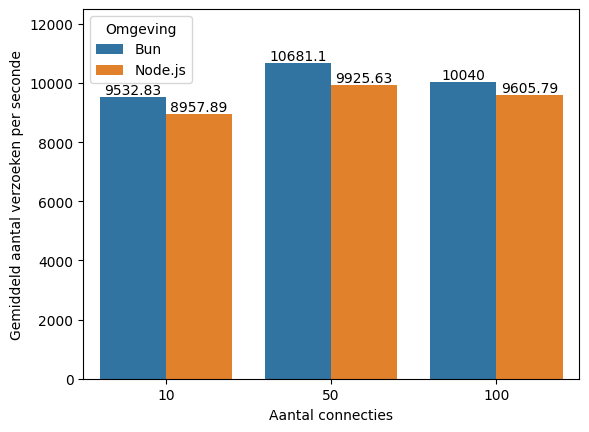
\includegraphics[width=0.7\columnwidth]{graphics/GetPostgresVerzoeken.png}
    \caption[Aantal verzoeken per seconde GET verzoek met PostgreSQL]{\label{fig:getaantalverzoekenpostgres}Visuele voorstelling gemiddeld aantal verzoeken per seconde bij het ophalen van de onderwerpen met PostgreSQL.}
  \end{figure}
  \begin{figure}[H]
    \centering
    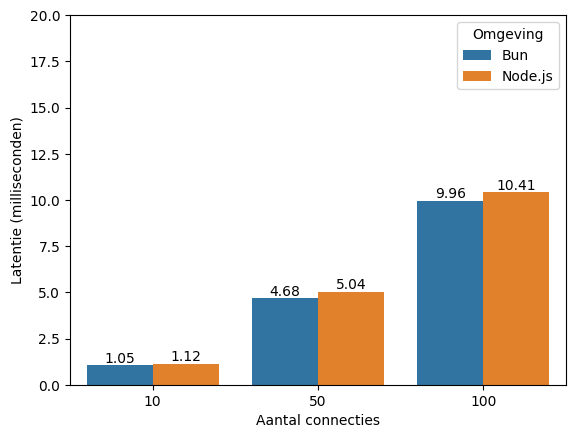
\includegraphics[width=0.7\columnwidth]{graphics/GetPostgresLatentie.png}
    \caption[Latentie GET verzoek met PostgreSQL]{\label{fig:getaantallatentienpostgres}Visuele voorstelling gemiddelde latentie bij het ophalen van de onderwerpen met PostgreSQL.}
  \end{figure}
  \begin{figure}[H]
    \centering
    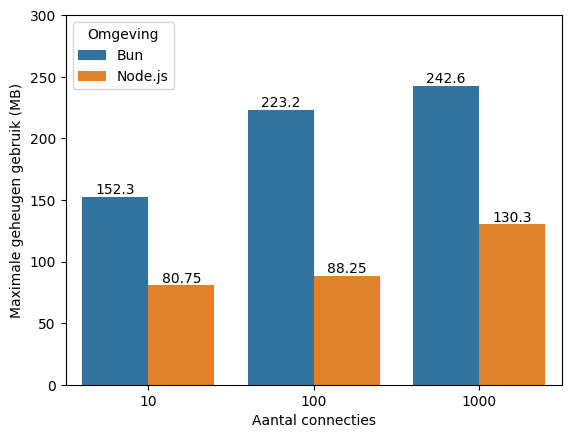
\includegraphics[width=0.7\columnwidth]{graphics/GetPostgresRAM.png}
    \caption[Geheugengebruik GET verzoek met PostgreSQL]{\label{fig:getgeheugenpostgres}Visuele voorstelling maximale geheugen gebruik bij het ophalen van de onderwerpen met PostgreSQL.}
  \end{figure}
  \begin{figure}[H]
    \centering
    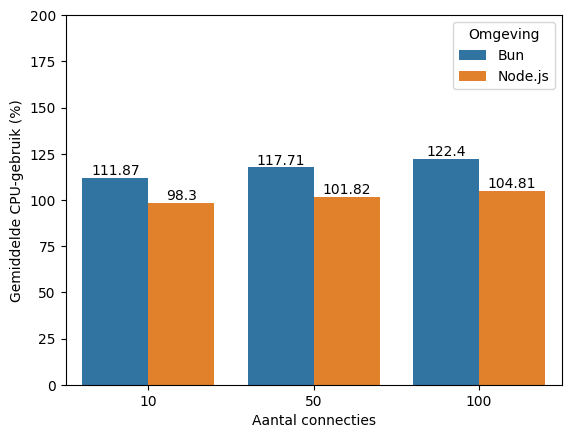
\includegraphics[width=0.7\columnwidth]{graphics/GetPostgresCpu.png}
    \caption[CPU-gebruik GET verzoek met PostgreSQL]{\label{fig:getcpupostgres}Visuele voorstelling gemiddeld CPU-gebruik bij het ophalen van de onderwerpen met PostgreSQL.}
  \end{figure}

In tabel \ref{tab:postbombardierpostgres} kunnen de resultaten gezien worden van de metingen waarbij 
een gebruiker een recensie schrijft over een bepaald onderwerp door gebruik van een POST verzoek en de PostgreSQL databank.
Hierbij scoort Bun consistent beter dan Node.js bij de latentie en het aantal verzoeken.
Zo heeft Bun bij 10 connecties een gemiddelde van 5433.39 aantal verzoeken per seconde met een latentie van 1.84 milliseconden. 
Dit tegenover Node.js met een gemiddelde van 5221.94 verzoeken per seconde en een latentie van 1.91 milliseconden.
Deze trend zet zich voort bij zowel 50 als 100 gelijktijdige connecties.
Hierbij heeft Node.js ook een substantieel grotere standaardafwijking voor de latentie die vooral merkbaar is bij 100 gelijktijdige connecties.
Op vlak van middelengebruik is er ook hier een verschil. Echter scoort Node.js hierbij beter dan Bun.
Zo heeft het bijvoorbeeld bij 100 connecties een maximaal geheugengebruik van 146.4MB en een gemiddeld CPU-gebruik van 104.75\%.
Bij Bun is dit hoger met een geheugengebruik van 179.2MB en een gemiddeld CPU-gebruik van 118.79\%.
In figuren \ref{fig:postaantalverzoekenpostgres}, \ref{fig:postaantallatentiepostgres}, \ref{fig:postgeheugenpostgres} en \ref{fig:postcpupostgres} kunnen de visuele voorstellingen 
voor respectievelijk het aantal verzoeken per seconde, het aantal latentie, het maximale geheugengebruik en het gemiddeld CPU-gebruik worden gevonden.
\begin{table}[H]
  \tabcolsep=0.13cm
  \begin{tabular}{|c|cccccc|}
  \hline
  \multicolumn{1}{|l|}{}                                                                     & \multicolumn{1}{l}{} & Bun     & \multicolumn{1}{l|}{}    & \multicolumn{1}{l}{} & \multicolumn{1}{l}{Node.js} & \multicolumn{1}{l|}{} \\ \hline
  Aantal connecties                                                                          & 10                   & 50      & \multicolumn{1}{c|}{100} & 10                   & 50                          & 100                   \\ \hline
  \begin{tabular}[c]{@{}c@{}}Gemiddeld aantal \\ verzoeken per seconde\end{tabular}          & 5433.39              & 6098.80 & 6170                     & 5221.94              & 5864.77                     & 5785.76               \\ \cline{1-1}
  \begin{tabular}[c]{@{}c@{}}Standaardafwijking aantal \\ verzoeken per seconde\end{tabular} & 1398.06              & 2151.57 & 2186.09                  & 1237.90              & 1866.52                     & 2023.42               \\ \cline{1-1}
  \begin{tabular}[c]{@{}c@{}}Latentie \\ (milliseconden)\end{tabular}                        & 1.84                 & 8.20    & 16.22                    & 1.91                 & 8.53                        & 17.30                 \\ \cline{1-1}
  \begin{tabular}[c]{@{}c@{}}Standaardafwijking\\ latentie\\ (milliseconden)\end{tabular}    & 0.97                 & 2.32    & 3.26                     & 0.9                  & 2.71                        & 7.79                  \\ \cline{1-1}
  \begin{tabular}[c]{@{}c@{}}Maximale \\ geheugengebruik \\ (MB)\end{tabular}                & 154.5                & 168.6   & 179.2                    & 142.9                & 149.6                       & 146.4                 \\ \cline{1-1}
  \begin{tabular}[c]{@{}c@{}}Gemiddeld\\ CPU-gebruik\\ (\%)\end{tabular}                     & 102.36               & 116.99  & 118.79                   & 91.76                & 103.15                      & 104.45                \\ \hline
  \end{tabular}
  \caption[Resultaten POST verzoek met PostgreSQL]{\label{tab:postbombardierpostgres}Resultaten metingen waarbij door een bepaalde gebruiker een recensie over een onderwerp werd gemaakt in de PostgreSQL database met een POST request.}
  \end{table}

  \begin{figure}[H]
    \centering
    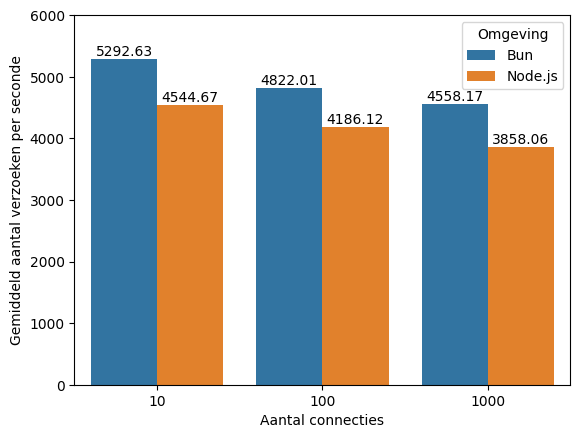
\includegraphics[width=0.7\columnwidth]{graphics/PostPostgresVerzoeken.png}
    \caption[Aantal verzoeken per seconde POST verzoek met PostgreSQL]{\label{fig:postaantalverzoekenpostgres}Visuele voorstelling gemiddeld aantal verzoeken per seconde bij het maken van een recensie met PostgreSQL.}
  \end{figure}
  \begin{figure}[H]
    \centering
    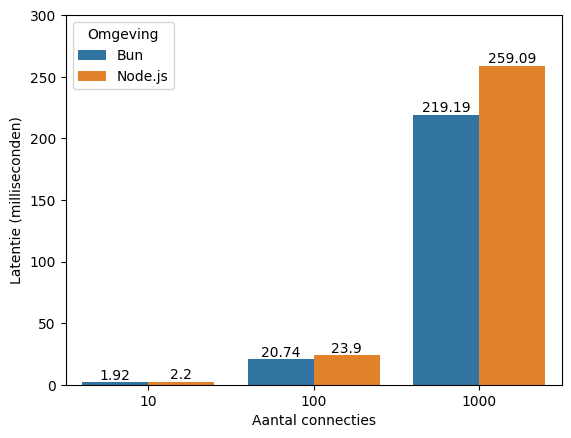
\includegraphics[width=0.7\columnwidth]{graphics/PostPostgresLatentie.png}
    \caption[Latentie POST verzoek met PostgreSQL]{\label{fig:postaantallatentiepostgres}Visuele voorstelling gemiddelde latentie bij het maken van een recensie met PostgreSQL.}
  \end{figure}
  \begin{figure}[H]
    \centering
    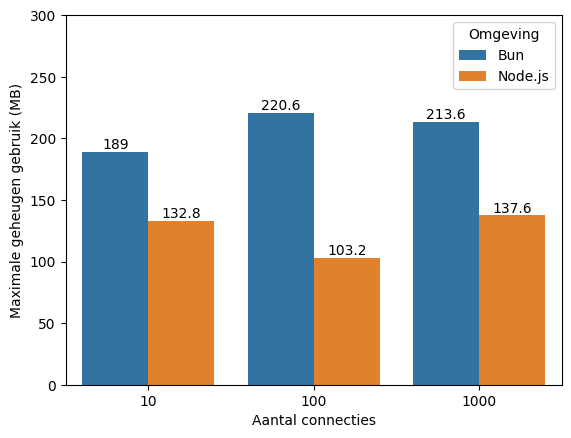
\includegraphics[width=0.7\columnwidth]{graphics/PostPostgresRAM.png}
    \caption[Geheugengebruik POST verzoek met PostgreSQL]{\label{fig:postgeheugenpostgres}Visuele voorstelling maximale geheugen gebruik bij het maken van een recensie met PostgreSQL.}
  \end{figure}
  \begin{figure}[H]
    \centering
    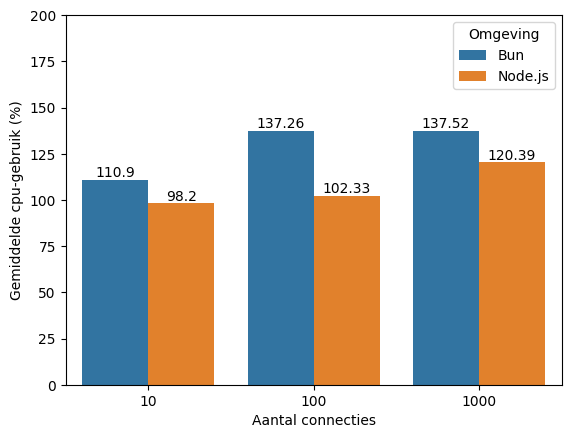
\includegraphics[width=0.7\columnwidth]{graphics/PostMySqlCpu.png}
    \caption[CPU-gebruik POST verzoek met PostgreSQL]{\label{fig:postcpupostgres}Visuele voorstelling gemiddeld CPU-gebruik bij het maken van een recensie met PostgreSQL.}
  \end{figure}
\subsection{Discussie}
Aan de hand van de QuickSort algoritme resultaten kan het standpunt dat Bun computationeel sneller is ondersteund worden.
Zo was de gemiddelde uitvoeringstijd van Bun gemiddeld 2.21 keer sneller dan Node.js en lag het middelengebruik bij Bun ook lager. Deze snellere uitvoeringstijd komt door de
het gebruik van de JavaScriptScore engine in Bun waarbij geoptimaliseerde machine code wordt geproduceerd in 
samenwerking met 3 JIT compilers en een Low-Level interpreter.
Deze snelheid is niet enkel zichtbaar bij het algoritme, maar ook bij de installatietijd van de packages.
Zo is Bun met een gemiddelde installatietijd van 24,9 milliseconden 24,5 keer sneller is dan Node.js met een 
gemiddelde installatietijd van 610,1 milliseconden. Dit kan een groot verschil betekenen op vlak van efficiëntie in projecten 
met een groot aantal packages.
Met behulp van de recensie applicatie kan er ook gekeken worden naar de performantie bij I/O-taken.
In de metingen werd hiervoor een GET en POST endpoint opengezet waarbij telkens met een MySQL database en een PostgreSQL database de metingen werden uitgevoerd.
Bij het ophalen van data scoort Bun bij zowel de MySQL database als de PostgreSQL database telkens beter dan Node.js op vlak van het gemiddeld aantal verzoeken per seconde en de latentie.
Het verschil in aantal verzoeken per seconde toont aan dat Bun een grotere capaciteit voor verzoeken heeft bij het ophalen van data.
De latentie toont aan dat Bun sneller de opgehaalde data kan teruggeven. Echter komen deze voordelen met een prijs. 
Zo heeft Bun telkens een groter gebruik van middelen tegenover Node.js wat aantoont dat Node.js efficiënter is op vlak van geheugen management en CPU-management.
Bij het invoegen van data was er een gelijkaardige situatie. 
Bij de MySQL databank presteert Bun beter dan Node.js, zowel wat betreft het gemiddelde aantal verzoeken als de latentie 
bij 50 en 100 gelijktijdige connecties.
Echter zet dit zich niet voort in het middelengebruik waarbij Bun telkens weer meer middelen gebruikt dan Node.js.
Bij de PostgreSQL database scoort Bun beter bij 10,50 en 100 gelijktijdige connecties wat betreft latentie en verzoeken 
per seconde. Echter, om deze resultaten te behalen, verbruikt Bun ook weer meer middelen.
Op basis van deze bevindingen kunnen verschillende conclusies worden getrokken. 
Zo kunnen applicaties met complexe algoritmes en calculaties beter kiezen voor Bun. 
Deze kan door middel van zijn geoptimaliseerde machine code de calculaties sneller uitvoeren dan Node.js.
Bij I/O-taken moet er echter een afweging gemaakt worden. Zo is Bun sneller voor het ophalen en invoegen van data.
Echter komt dit ten koste van een hoger middelengebruik op vlak van geheugen- en CPU-gebruik. 
Indien de server hardware over voldoende middelen beschikt kan Bun gebruikt worden voor een snellere verwerking binnen de applicatie.

